\chapter{Something New}
\label{newThing}
In this chapter, we focus on the TETRIS method, mentioned in section \ref{tetris}. Specifically, we focus on the reordering technique briefly described in subsection \ref{reordering}.

\section{Pruned Matrix}
\label{sec:pruned_matrix}

To discuss the reordering algorithms, we first need to define what exactly we mean by a pruned matrix. A pruned matrix is the result of applying the mask matrix to the original weight matrix. Here, applying means element-wise multiplication.

The mask matrix is a binary matrix that has the same dimensions as the weight matrix. Ones in the mask matrix determine which elements of the weight matrix will be kept, and zeros determine which elements will be pruned. An example of a mask matrix $M$ for a weight matrix $A$, resulting in a pruned matrix $P$, is shown in figure \ref{fig:pruned}. We will use these example matrices later on.

\begin{figure}[h]
    % inserting the centered image in the correct size
    \centerline{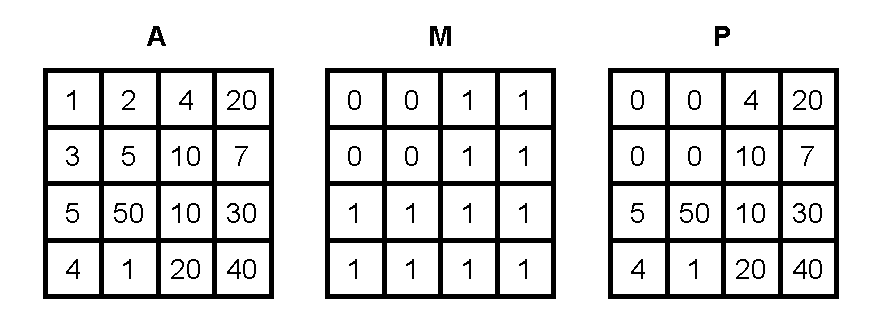
\includegraphics[width=0.8\textwidth]{images/pruned}}
    %image description
    \caption[Pruned matrix]{Pruned matrix $P$ is the result of element-wise multiplication of mask matrix $M$ and weight matrix $A$}
    %id of the image, which can be used to reference the image
    \label{fig:pruned}
\end{figure}

The purpose of the pruning algorithm is to find a mask matrix that minimizes the norm of the pruned matrix while maintaining several rules, for example, pruning only elements lower in value than some constant. The norm of a matrix is a function that assigns a number to the matrix. We use this norm as a measure of the quality of the mask matrix.

For example, the norm of the matrix can be the sum of the absolute values of the elements of the matrix. This norm is called the $L_1$ norm, and we will use it throughout this chapter.

\section{Reordering Algorithm}

In general, the reordering algorithm from the TETRIS method works in iterations to find permutations in each dimension, optimizing the norm of the pruned matrix. For simplicity, we consider just one dimension. For example, we have a two-dimensional weight matrix, and we want to find a permutation of the rows that maximizes the norm of the pruned matrix.

In one iteration, the algorithm generates the mask using the given pruning method. The aim is to perform structural pruning, so the zeros in the mask matrix form structured regions, for example, $2\times2$ matrices. Then, it tries to find the permutation that maximizes the norm of the pruned matrix using the calculated mask.

The second step is done using a greedy algorithm that swaps two indexes in the permutation that mostly increases the norm of the pruned matrix until convergence. This algorithm finds a local maximum of the norm of the pruned matrix, but it is not guaranteed to find the global maximum.

We will develop an algorithm that is guaranteed to find the optimal permutation in the second step.

\section{Permutation as a Bipartite Graph}
\label{sec:permutation_as_graph}

To avoid the greedy algorithm that performs locally optimal swaps, we will represent the problem on a bipartite graph. To do this, first, we observe how to represent a permutation as a graph.

Any permutation of elements from $1$ to $n$ can be represented as a bipartite graph. The graph has two sets of vertices, $A$ and $B$, each of size $n$. Both sets have vertices representing numbers from $1$ to $n$. The edges of the graph represent the permutation. If there is an edge between vertex $i$ from set $A$ and vertex $j$ from set $B$, it means that the $i$-th element of the permutation is $j$. For example, the permutation $[2, 4, 1, 3, 5]$ can be represented as a bipartite graph in figure \ref{fig:permutation_graph}.

\begin{figure}[h]
    % inserting the centered image in the correct size
    \centerline{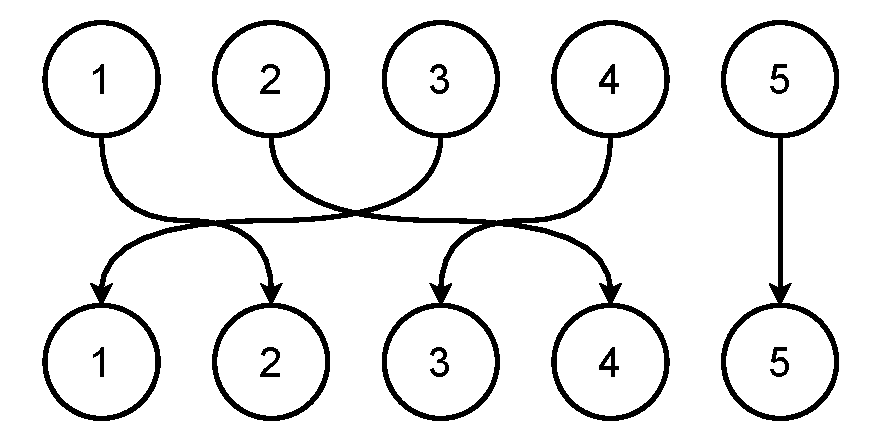
\includegraphics[width=0.8\textwidth]{images/permutation_graph}}
    %image description
    \caption[Bipartite graph representing permutation]{Bipartite graph representing permutation $[2, 4, 1, 3, 5]$}
    %id of the image, which can be used to reference the image
    \label{fig:permutation_graph}
\end{figure}

In a more detailed view, the permutation not only represents a bipartite graph but also a perfect matching in the bipartite graph. From another perspective, a given bipartite graph with two sets of vertices of the same size $n$ and a set of edges represents a set of permutations of elements from $1$ to $n$.

Specifically, the set of perfect matchings in the graph corresponds to a set of permutations of elements from $1$ to $n$. A fully connected bipartite graph represents all possible permutations of elements from $1$ to $n$.

\section{Reordering Algorithm Using Bipartite Graph}

Any reordering algorithm ultimately computes a permutation of the rows of the weight matrix. Therefore, the set of possible outputs of a reordering algorithm is the set of all permutations of rows.

As shown in the previous section \ref{sec:permutation_as_graph}, this set can be represented as a fully connected bipartite graph, where each perfect matching represents a unique feasible output of the reordering algorithm.

\section{Finding the Optimal Permutation}

The purpose of the reordering algorithm is to find the optimal permutation of the rows of the weight matrix. Therefore, our algorithm will choose one specific perfect matching in the fully connected bipartite graph.

Our goal is to find the perfect matching (which corresponds to the desired permutation) that maximizes the norm of the pruned matrix. In order to do so, we need a way to transfer the changes in the norm caused by the permutation to the bipartite graph representation.

Each edge $(i, j)$ in the bipartite graph represents an exchange of rows $i$ and $j$ in the weight matrix. We can calculate the change in the norm $\delta$ of the pruned matrix caused by this exchange. To calculate $\delta$, we simply sum the values of elements that are moved from the pruned to the unpruned part of the matrix and subtract the values of elements that are moved from the unpruned to the pruned part of the matrix.

To capture the change in the norm in the bipartite graph, we assign the value of $\delta$ to the edge $(i, j)$. This way, we have a weighted bipartite graph, where the weight of the edge $(i, j)$ represents the change in the norm of the pruned matrix caused by the exchange of rows $i$ and $j$. The sum of the weights of the edges in the perfect matching represents the norm of the pruned matrix after applying the permutation.

An example of weight assignments to the edges corresponding to the swaps on the example matrix from section \ref{sec:pruned_matrix} shown in \ref{fig:norm-change} is shown in figure \ref{fig:weighted}.

\begin{figure}[h]
    % inserting the centered image in the correct size
    \centerline{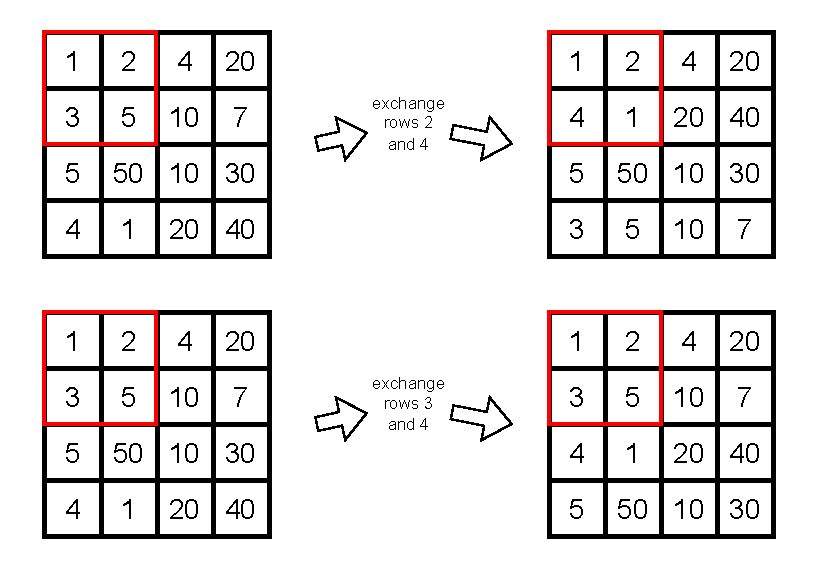
\includegraphics[width=0.8\textwidth]{images/norm-change}}
    %image description
    \caption[Swaps on the matrix]{Example swaps on the matrix from section \ref{sec:pruned_matrix}, the red squares represent the pruned elements}
    %id of the image, which can be used to reference the image
    \label{fig:norm-change}
\end{figure}

\begin{figure}[h]
    % inserting the centered image in the correct size
    \centerline{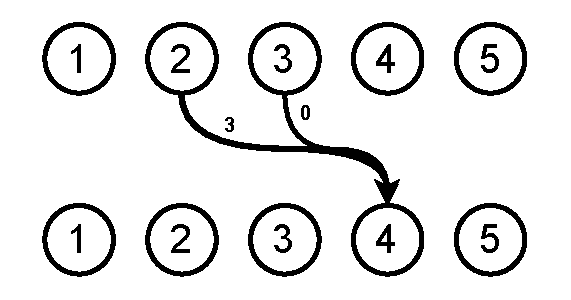
\includegraphics[width=0.8\textwidth]{images/weighted}}
    %image description
    \caption[Weighted bipartite graph]{Weighted bipartite graph representing the change in the norm of the pruned matrix caused by the swaps in figure \ref{fig:norm-change}}
    %id of the image, which can be used to reference the image
    \label{fig:weighted}
\end{figure}

\section{Optimal Permutation as Maximum Weight Matching}
In previous sections, we demonstrated every tool needed to construct an algorithm that finds the optimal permutation of the rows of the weight matrix. Effectively, we reduced the problem of finding the optimal permutation to the problem of finding the maximum weight perfect matching in a weighted bipartite graph.

The maximum weight perfect matching is a well-known problem in graph theory and has a few known polynomial-time algorithms. One of the algorithms with the best time complexity is the Hungarian algorithm, with a time complexity of $O(n^3)$. There is no known algorithm with better time complexity for this problem.

However, there are some algorithms with better time complexity for specific cases. Also, there are approximation algorithms that trade off optimality for better time complexity, such as the local search algorithm.
